\documentclass[a4paper,twoside, openany,11pt]{book}
\usepackage{import}
\import{C:/Users/adrie/OneDrive/Programmation/LATEX/0_macro/Macro_2018_01_06/}{ensae_memoire.tex}

\programmationCPP

\newcommand{\PDGtitre}{Projet de C++ 2A}
\newcommand{\PDGsoustitre}{Réalisation d'un RPG Pokémon}
\newcommand{\PDGbasgauche}{MEILAC Adrien\\Langlois Romain}
\newcommand{\PDGbasdroit}{Encadrant:\\Jean-Baptiste Yunès}

\newcommand{\Floor}[1]{\left\lfloor #1 \right\rfloor}

\begin{document}
\vspace*{0.5cm}

\section*{Introduction}
\phantomsection
\addcontentsline{toc}{section}{Introduction}
\vspace*{0.5cm}

Nous avons depuis notre enfance été plongés dans le monde des RPG. Si nos goûts spécifiques ont pu varier, nous partageons néanmoins une passion toute particulière pour ces jeux souvent inimitables. Nous avons ainsi dans le cadre de ce projet décidé de la faire partager en reprenant un RPG incontournable, Pokémon. 
\vspace*{0.5cm}

Pokemon a été créé en 1996 par Satoshi Tajiri. Cette franchise a réalisé des records de ventes dans l'histoire des jeux vidéos dès ses premières éditions Rouge et Bleu, vendues à plus de 30 millions d'exemplaires. Aujourd'hui, Pokémon est exploité sous forme d'animés, de mangas, de jeux de cartes et plus récemment d'application mobile avec Pokémon Go et génère plus de 3.3 milliard de chiffre d'affaires (année 2016). \\
Nous avons entrepris de coder notre RPG en C++ avec une interface graphique en C. Nous avons également utilisé en Python pour pouvoir créer des bases de données propres à partir de données brutes. Nous avons choisi d’utiliser la bibliothèque SDL (associée avec SDL Image et SDL ttf) pour l'interface graphique car cette dernière contient des fonctions adaptées à la création de jeux de plateforme. 
\vspace*{0.5cm}

La réalisation de ce jeu représentait un immense défi que nous avons décidé de relever. Notre projet Pokémon est une version épurée qui s'inspire à l'original mais qui rappellera des souvenirs aux connaisseurs.
\vspace*{1cm}

\begin{minipage}{0.45\textwidth}

\includegraphics[scale = 0.42]{Images/Psykokwak.png}
\end{minipage}
\begin{minipage}{0.45\textwidth}

\includegraphics[scale = 0.26]{Images/Pikachu.png}
\end{minipage}

\newpage 
\pagestyle{PageNormale}

\section{Description de l'utilisation du jeu}
Pour pouvoir rester au plus proche du jeu original, nous avons utilisé des bases de données créées par les fans sur le site de Pokémon essentials. Nous en avons extrait divers éléments graphiques ainsi que des polices de caractère et des fichiers contenant de vraies données sur les Pokémon. C'est pourquoi notre  interface graphique et celle du vrai jeu se ressemblent beaucoup. 

\subsection{Présentation de l'interface de combat}
\begin{figure}[!h]
\begin{minipage}{0.49\textwidth}
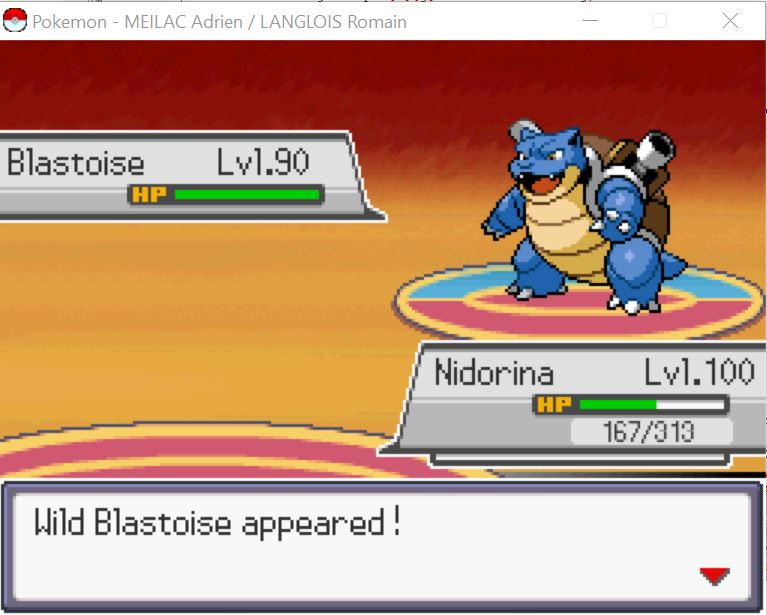
\includegraphics[scale = 0.6]{Images/combat_start.jpg}
\end{minipage}
\begin{minipage}{0.49\textwidth}
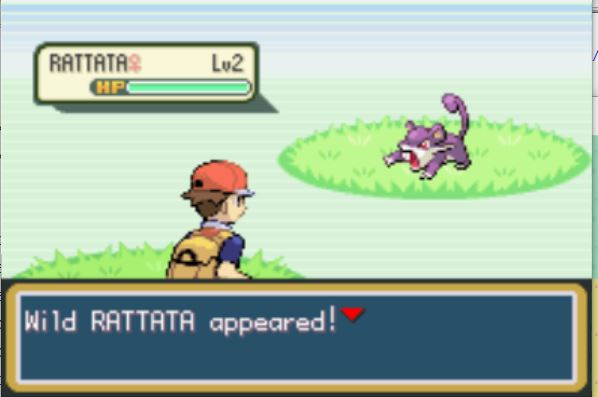
\includegraphics[scale = 0.84]{Images/vrai_jeu_combat_start.jpg}
\end{minipage}
\caption{Début de combat}
\end{figure}

Prenons par exemple la rencontre d'un pokémon aléatoire, générée par une loi binomiale lors du déplacement sur la carte. Une fenêtre de dialogue va apparaître, ainsi que l'arrière-plan de combat et également le Pokémon ennemi. Une pression de la touche entrée permet alors d'afficher le menu contextuel de combat.

\begin{figure}[!h]
\begin{minipage}{0.49\textwidth}
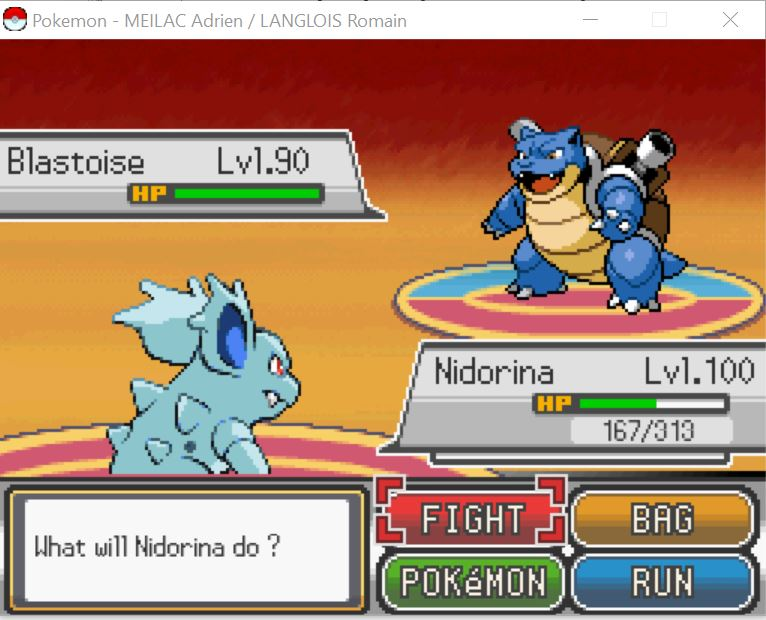
\includegraphics[scale = 0.6]{Images/mainMenu.jpg}
\end{minipage}
\begin{minipage}{0.49\textwidth}
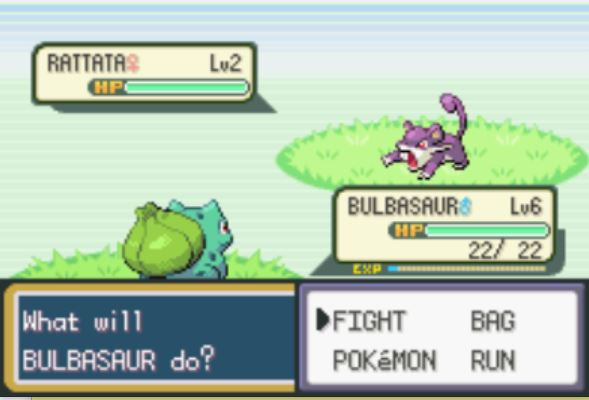
\includegraphics[scale = 0.84]{Images/vrai_jeu_mainMenu.jpg}
\end{minipage}
\caption{Menu principal}
\end{figure}


Dans ce menu, comme dans le jeu original, le joueur a le choix entre accéder à son inventaire (BAG), choisir son pokémon destiné à combattre (POKEMON), s'enfuir (RUN), ou alors attaquer (FIGHT).

Si le joueur décide de s'enfuir, il revient sur la map générale et ses Pokémon gardent les dégâts qu'ils ont subis lors du combat. Cependant, nous n'avons pas eu le temps de conserver la position du joueur lors du lancement du combat, c'est pourquoi ce dernier est remis à sa position initiale. 

\begin{figure}[!h]
\begin{minipage}{0.49\textwidth}
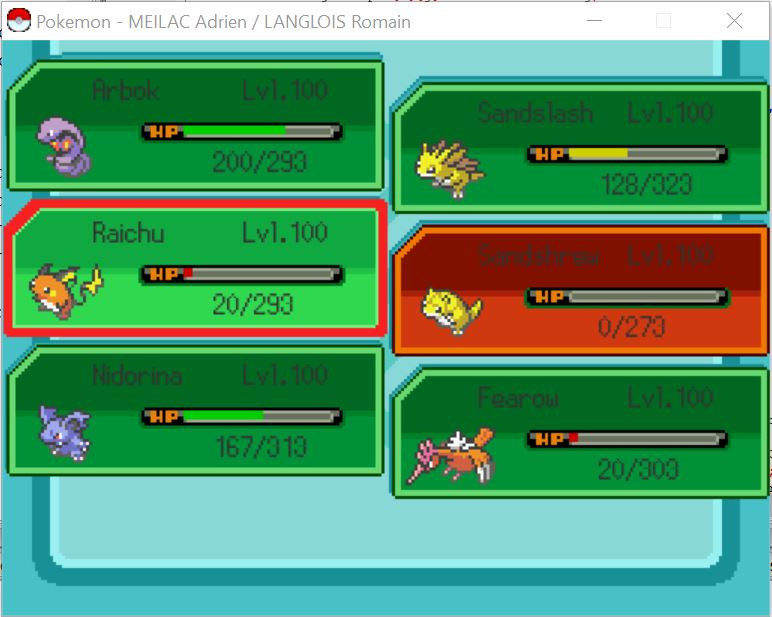
\includegraphics[scale = 0.6]{Images/swapMenu.jpg}
\end{minipage}
\begin{minipage}{0.49\textwidth}
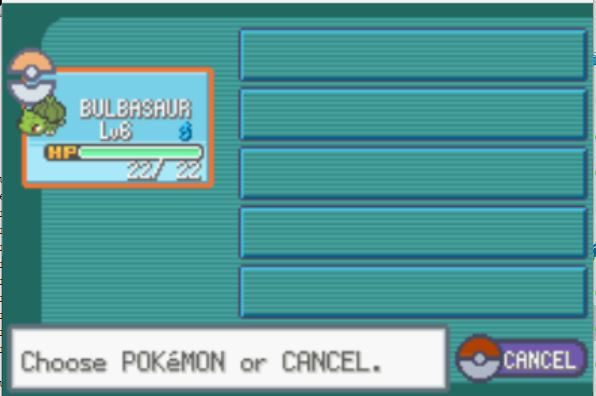
\includegraphics[scale = 0.84]{Images/vrai_jeu_swapMenu.jpg}
\end{minipage}
\caption{Menu du dresseur}
\end{figure}

Le menu Pokémon, appelé menu du dresseur, permet au joueur de choisir le Pokémon qui va combattre, et de voir l'état de santé ainsi que le niveau de ses Pokémon. Les Pokémon morts apparaissent en rouge et ne peuvent être sélectionnés pour combattre. 

Nous avons réalisé un effet visuel sur les barres d'HP. Leur longueur est ainsi adaptée au pourcentage de leur vie restant, et la couleur change: rouge en-dessous de 20\%, orange entre 20 et 50\%, et vert au-delà. Cet effet est aussi visible sur l'écran de combat principal, ce qui rend le combat plus interactif. 

\begin{figure}[!h]
\begin{minipage}{0.49\textwidth}
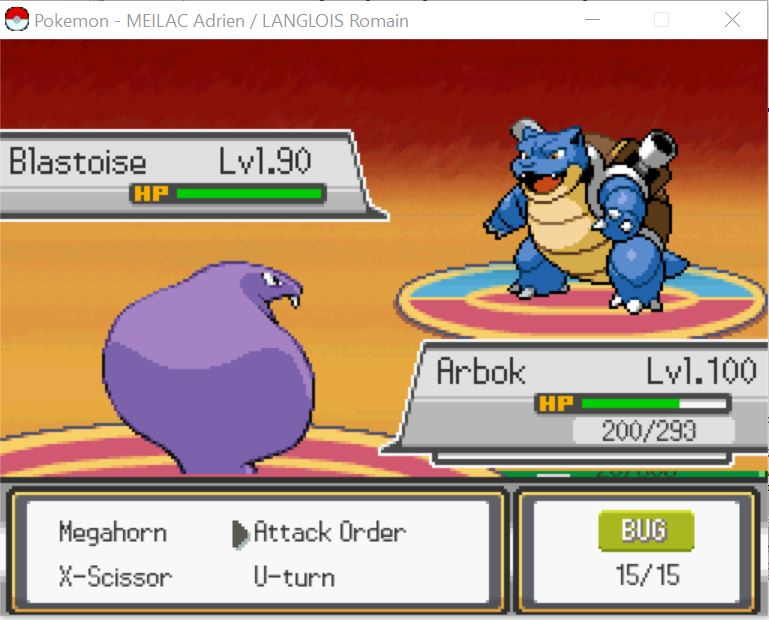
\includegraphics[scale = 0.6]{Images/fightMenu.jpg}
\end{minipage}
\begin{minipage}{0.49\textwidth}
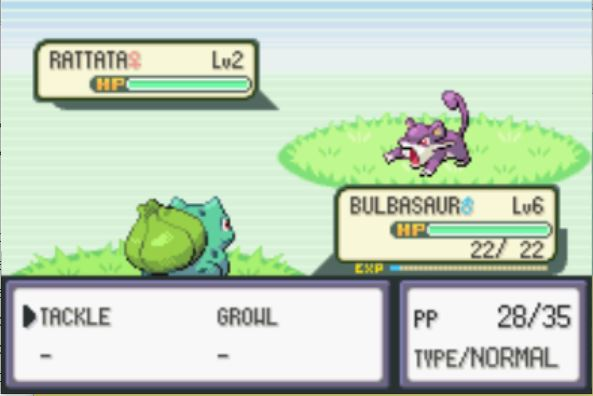
\includegraphics[scale = 0.84]{Images/vrai_jeu_fightMenu.jpg}
\end{minipage}
\caption{Menu de combat}
\end{figure}


Si le combat est adopté, un menu comprenant les diverses capacités disponibles pour le pokémon retenu apparait. Lorsque le joueur sélectionne une capacité à l'aide du curseur, il peut voir son type ainsi que ses Points de puissance (PP). Le combat se déroule ensuite au tour par tour en respectant les priorités d'ordre d'attaque entre les Pokémon. A chaque étape le menu est remplacé par une fenêtre de dialogue indiquant l'attaque utilisée. On voit alors le Pokemon touché perdre ses points de vie progressivement. Certaines capacités, comme Hail (Grêle dans le jeu français) de Nidorina, ne font pas de dégâts à l'adversaire mais ont un effet sur le temps du terrain, qui va se répercuter durant plusieurs tours à l'aide d'un message dans la boîte de dialogue.

\begin{figure}[!h]
\begin{minipage}{0.49\textwidth}
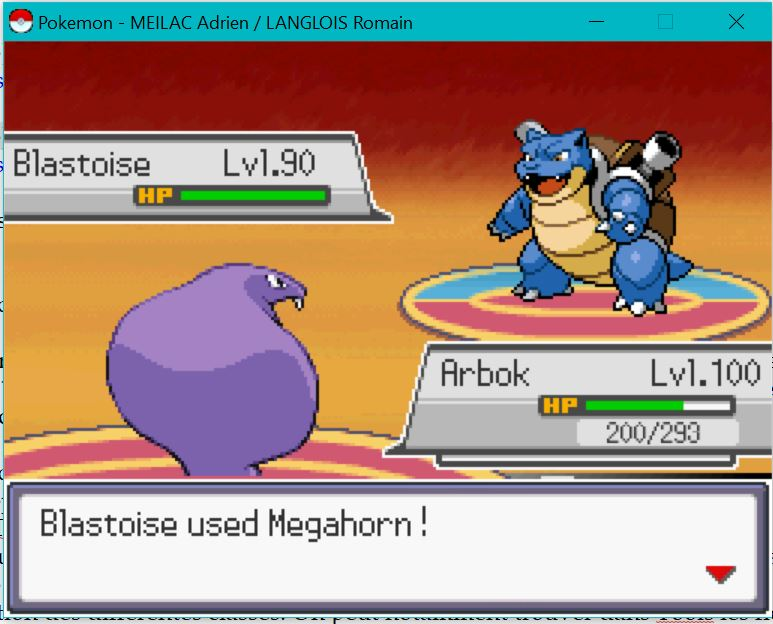
\includegraphics[scale = 0.6]{Images/useMove.jpg}
\end{minipage}
\begin{minipage}{0.49\textwidth}
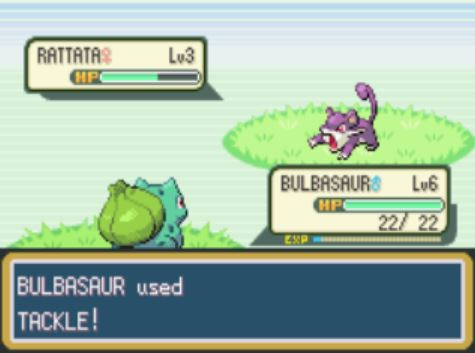
\includegraphics[scale = 0.84]{Images/vrai_jeu_useMove.jpg}
\end{minipage}
\caption{Joueur sur la carte Pokémon}
\end{figure}

Certains des Pokemon meurent ou terrassent leur adversaire en un seul tour. C'est un choix volontaire de notre part, nous avons pensé que la démonstration serait plus fluide s'il y avait possibilité d'observer directement les conséquences d'une victoire ou d'une défaite. Ces paramètres sont modifiables dans le fichier Player\_Pokemon.txt.\\

Le pokémon sélectionné par défaut, Nidorina, possède approximativement les stats de son adversaire. Le Pokemon Arbok a été configuré avec des statistiques largement surévalué pour tester les cas de victoires et les autres Pokemon ont des statistiques largement sous évalué pour tester les cas d'échec.  

Dans le cas d'une victoire, le Pokémon vainqueur reçoit des points d'expérience (exp) dans une fenêtre contextuelle, puis le joueur revient sur la map. Dans le cas où Pokemon du joueur est terrassé, ce dernier se voit contraint de sélectionner un autre Pokemon dans le menu de dressage pour pouvoir continuer le combat. Si tous les Pokemon décèdent, une boite de dialogue Game Over apparait, il convient alors de fermer le jeu pour le relancer.

\subsection{La carte du jeu}

\begin{figure}[!h]
\begin{minipage}{0.49\textwidth}
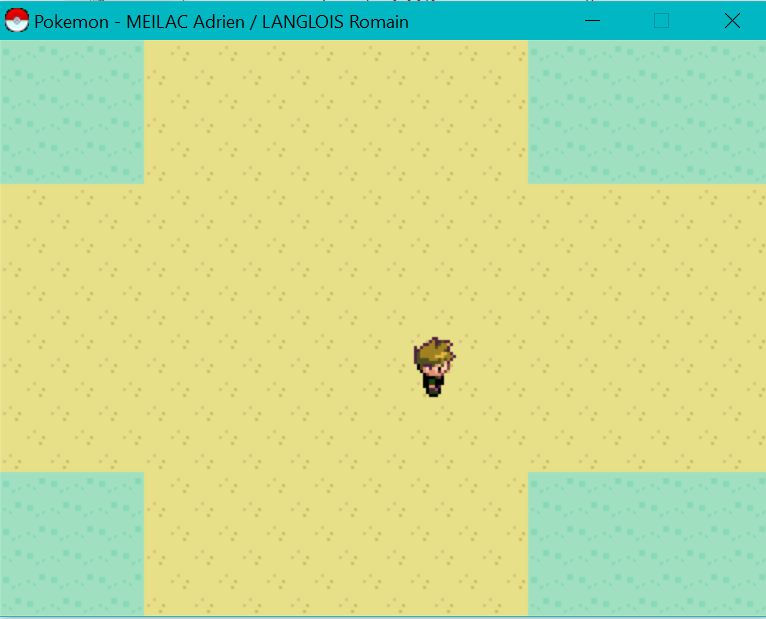
\includegraphics[scale = 0.6]{Images/map.jpg}
\end{minipage}
\begin{minipage}{0.49\textwidth}
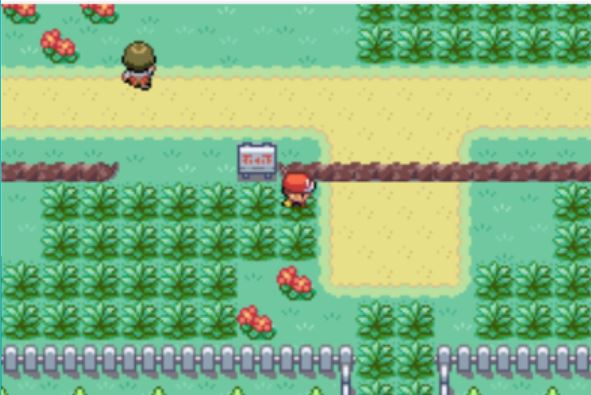
\includegraphics[scale = 0.84]{Images/vrai_jeu_map.jpg}
\end{minipage}
\caption{Joueur sur la carte Pokémon}
\end{figure}


Le joueur est également libre de se déplacer sur la map quand il n'est pas en combat. La pression de la touche Espace lui permet d'afficher un menu. Il peut par exemple afficher ses différents Pokemon disponibles ou alors revenir sur la map à l'aide du bouton Exit. Une courte description de chaque option est également disponible.


\begin{figure}[!h]
\begin{minipage}{0.49\textwidth}
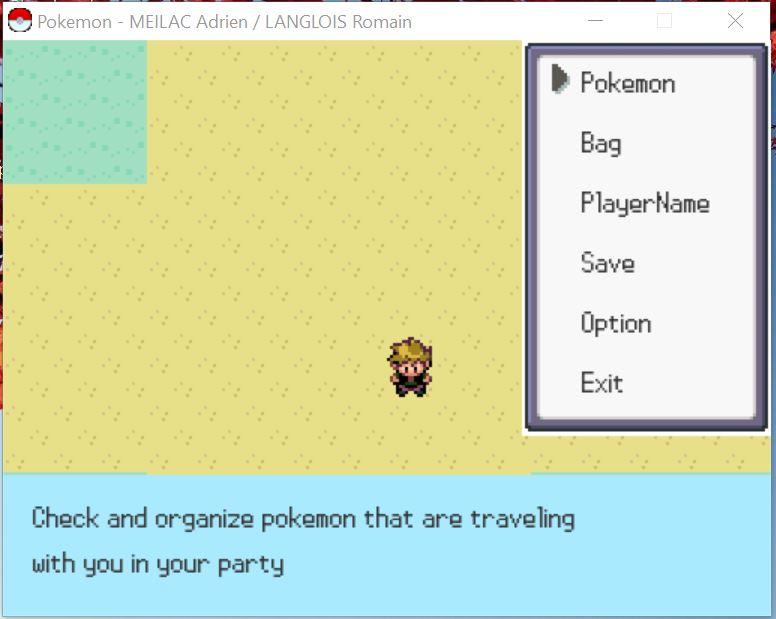
\includegraphics[scale = 0.6]{Images/fieldMenu.jpg}
\end{minipage}
\begin{minipage}{0.49\textwidth}
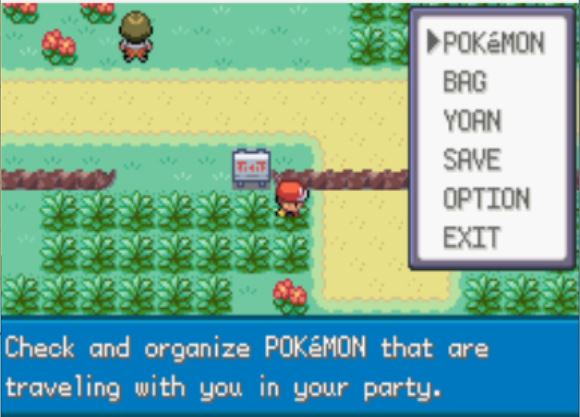
\includegraphics[scale = 0.84]{Images/vrai_jeu_fieldMenu.jpg}
\end{minipage}
\caption{Menu sur le terrain}
\end{figure}

Nous n'avons pas réalisé l'inventaire ni les autres options de ce menu du fait d'un manque de temps, le code existant ayant déjà nécessité beaucoup de lignes, mais nous disposons désormais de tous les outils nécessaires pour réaliser ces améliorations. Pour la même raison, nous n'avons laissé qu'une seule couche d'arrière-plan sur la map et n'avons pas eu le temps de gérer les déplacements de la carte, ni la liaison entre la carte et des lieux stockés dans les données, ni l'affichage des bâtiments.

\newpage

\section{Architecture générale du code}

D'après GitHub, notre code est composé de 35 fichier .cpp et de 23 fichier .h, et notre projet contient environ 14 000 lignes. Pour ne pas se perdre dans notre projet, nous avons donc essayé de hiérarchiser au maximum notre code et de créer le namespace PKMN pour pouvoir reconnaître plus facilement nos fonctions. 

\begin{figure}[!h]\centering
\import{Graphiques/}{hierarchie_globale_projet.tex}
\caption{\label{ArchiGenerale}Schéma de l'architecture générale du projet}
\end{figure}

L'organigramme \ref{ArchiGenerale} illustre schématiquement les interactions entre les différentes parties de notre code. Lorsque le programme est lancé par l'utilisateur. Ce dernier va commencer par préparer les méthodes d'accès aux données (stockées dans le répertoire Tools) et va remplir la structure de nos données (la plupart des classes que nous avons écrites se trouvent dans Pokémon) avec les données stockées dans les répertoires Data et BackUp. 

Ces structures de données sont majoritairement composées d'accesseurs et permettent de modifier les données et de les sauvegarder via les méthodes d'accès. Nous avons essayé de les différentier des structures du jeu (qui correspond principalement aux fichiers BattleWildPokemon et main). Ces dernières utilisent les structures de données mais n'agissent pas directement sur les fichiers. 

De l'autre côté, l'utilisateur a uniquement accès aux commandes graphiques (stockées dans Graphics). Nous avons décider de les séparer de la structure du jeu pour :
\begin{itemize}
\item éviter d'avoir des fonctions trop longues,
\item  distinguer le cœur de notre code qui est en C++ alors que les fonctions graphiques sont en C
\item pouvoir utiliser les options avancées de classe qui sont incompatibles avec l'option extern C. 
\item avoir des fonctions graphiques qui ne touchent pas aux données et réalisent juste de l'affichage
\end{itemize}
Pour pouvoir réaliser une telle coupure, nous avons créé des fonctions graphiques qui prennent l'écran en paramètre et qui le remplissent. Elles fonctionnent avec des boucles infinies qui vont s’arrêter (soit parce que l'utilisateur a sélectionné un choix, soit spontanément dans le cas d'un effet aléatoire) et renvoyer un ''flag'' (codé sous forme de string ici) aux structures du jeu qui vont agir en fonction du flag reçu. Nous nous sommes servis du double buffering pour que l'utilisateur ne puisse pas voir les jointures entre nos différents affichages. 

Enfin notre programme rédige un log (stocké dans stdout.txt) qui nous permet de tracer les incohérences dans le gameplay. 

Le jeu en lui même est une boucle infinie qui s'arrête lorsque l'utilisateur ferme la fenêtre. 

\newpage

\section{Architecture détaillée et problèmes rencontrés}
Cette partie rentre plus en détail dans la manière dont notre code fonctionne et explique sa répartition dans les différents répertoires.


\subsection{Méthodes d'accès et de conversion des données (Tools)}
Tools contient tous les outils dont nous avons eu besoin lors de notre projet, qui ne sont pas directement relié au mécanisme de fonctionnement de notre jeu, mais qui permettre de simplifier la création des différentes classes. On peut notamment trouver dans Tools les fichiers (et leur header) suivants :

\begin{itemize}
\item \textbf{Table }: La totalité de nos fichiers sont des tableaux (avec comme délimiteurs '';''). C'est pourquoi il nous a paru essentiel de simplifier la lecture des fichiers en créant une classe qui les lirait. Cette classe est capable d'extraire une ligne, une colonne et surtout de donner un élément à partir de son nom de ligne et de son nom de colonne (surcharge de l'opérateur () car [] ne peut être surchargé qu'avec un argument). Afin de standardiser la saisie, nous avons décider que la lecture des tableaux donnerait uniquement des chaînes de caractères (et ne chercherait donc pas à donner des nombres). Cette classe nous a posé quelques problèmes lorsque nous avons essayé de l'utiliser en écriture.

\begin{figure}[!h]\centering
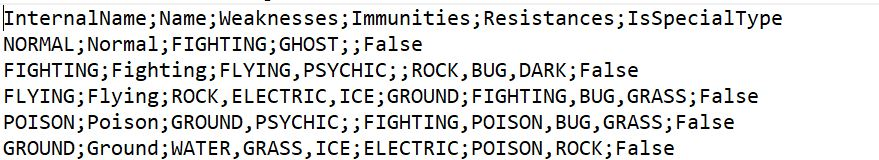
\includegraphics[scale = 0.84]{Images/fichierTexteExemple.jpg}
\caption{Exemple de fichier lu par Table}
\end{figure}

\item \textbf{VectorMethod} : Ce fichier contient des fonctions supplémentaires concernant les vecteurs. Notamment, un test vector\_in qui permet de dire si un élément est dans le vecteur, et une fonction qui permet de découper les chaînes de caractères. Cette dernière sert par exemple lors de la création des objets de type Table. 
\item \textbf{Conversion} contient une collection de fonctions permettant de convertir les objets d'un type à un autre. En effet, le compilateur MinGW fournit par notre IDE CodeBlocks ne nous laissait pas utiliser les fonction stoi, atoi stol ... qui permettent la conversion directe des types. Nous avons donc créé nos propres fonctions. Ces dernières sont généralement utilisées après la lecture des fichiers contenant des données pour convertir les std::string que la classe Table permet d'extraire (et donc de compenser le fait que Table ne soit composé que de std::string)

\item \textbf{Random} qui contient des fonctions plus simples pour faire appel à l'aléatoire. Nous avons eu des difficultés à utiliser la fonction std::uniform\_real\_distribution, c'est pourquoi nous avons créé une approximation de cette dernière à l'aide de rand()

\item  \textbf{StatSet} et \textbf{StatSetExt} sont des classes (la seconde héritant de la première) qui permettent de stocker les différentes statistiques de nos Pokémon. Lors de leur création, nous nous sommes aperçu que des arguments liés aux points de vie, d'attaque, de défense, d'attaque spéciale, de défense spéciale et de vitesse. Nous avons aussi mis dedans la formule permettant de calculer les statistiques d'un Pokémon. \\
Si on note
\begin{itemize}
\item \textbf{Niv}, le niveau d'un Pokémon, \\
\item \textbf{PV} sa vie maximum, \\
\item \textbf{Stat} la valeur de ses autres statistiques (Attaque Défense, Attaque Spéciale, Défense Spéciale, Vitesse) (cette valeur est celle qui est valable lorsque le Pokémon est soigné), \\
\item \textbf{IV} des paramètres pour chacune des statistiques (ces derniers varient entre 0 et 31, ils sont générés aléatoirement lors de la création d'un Pokémon, ils ne sont ni visibles ni modifiables),\\
\item \textbf{EV} des paramètres pour chacune des statistiques (ces derniers varient entre 0 et 255, ils valent 0 lors de la création d'un Pokémon et varient en fonction des combats effectués, ils ne sont pas visibles par l'utilisateur, mais ce dernier peut les modifier indirectement),\\
\item \textbf{Base} des paramètres pour chacune des statistiques traduisent l'influence de l'espèce sur un Pokémon,
\end{itemize}
alors les statistiques d'un Pokémon sont définies par :
\[
Stat = \Floor{\dfrac{2 * Base + IV + \Floor{\frac{EV}{4}} * Niv + 5}{100} * Nat}
\]
\[
PV =\Floor{\dfrac{2 * Base + IV + \Floor{\frac{EV}{4}} * Niv}{100}} + Niv + 10
\]
\end{itemize}

\subsection{Structures de données (Pokémon)}
Pokémon est un répertoire qui contient l'architecture des classes que nous remplissons lorsque le programme est lancé. La plupart des classes ont un constructeur qui prend en paramètre un nom interne d'objet dont les caractéristiques sont définies dans un ou plusieurs fichiers. Le constructeur va alors utiliser la fonction Table pour lire la ligne du fichier qui l’intéresse et construire l'objet, ce qui simplifie énormément la déclaration des classes. Nous avons fait notre code de tel sorte que les arguments des uns sont les noms internes des autres ce qui permet de créer automatiquement les objets associés. 

Par ailleurs, la plupart des objets ont une structure qui n'est pas aléatoire et qui est totalement déterminé par le nom interne de l'objet, nous avons donc surchargé les operateurs == entre un objet et un std::string pour simplifier les déclarations d'égalité et rendre le code plus lisible (cela permet d'écrire par exemple if(type == ''FIRE'') ...)

Voici une description des différentes classes :

\begin{itemize}
\item \textbf{Type} contient la classe codant le Type des Pokémon ou des attaques. Les méthodes les plus importantes de cette classes sont effectiveness qui donne l'efficacité d'un Type sur un autre (par exemple, une attaque de type Eau sera très efficace contre un Pokémon de Type Feu), ainsi que getPathImage qui permet de donner l'image à afficher pour indiquer le Type d'un Pokémon.
\item \textbf{Move} contient la classe codant les attaques des Pokémon. Elle est lié au fichier ''Data/Move.txt'' qui contient énormément d'argument, parfois très complexes. Nous n'avons donc pas tout utilisé. Move contient des objets issus des classes Flag, Target et DamageCategory qui correspondent à des effets particuliers liés au attaques. Ces classes offrent une gamme de test booléen pour éviter d'avoir à gérer des notations abstraites. 
\item  \textbf{Species} contient les arguments liés à l'espèce d'un Pokémon. Nous avons décidé de sauvegarder les mouvements que peut apprendre un Pokémon (en moyenne, une centaine) sous forme de string pour ne pas utiliser inutilement de la mémoire étant donné que seul 4 sont utilisés (et sont donc converti en Move dans la classe fille Pokémon). 
\item  \textbf{Pokémon} contient principalement les fonctions qui permettent de faire varier les statistiques des Pokémon. On lui associe 2 Types, 4 Attaques, ainsi que deux structures de statistiques, l'une étant l'état normal, et l'autre l'état actuel (En effet, si un Pokémon est blessé, il n'a pas sa vie au maximum, cette information est stockée dans l'état actuel. Toutefois, si il est soigné, il revient à son état normal. Cet état normal peut aussi jouer dans le calcul des dégâts, d'où l’intérêt de le sauvegarder comme un argument). 
\end{itemize}

\begin{figure}[!h]\centering
\import{Graphiques/}{hierarchie_des_classes_de_donnees.tex}
\caption{Hiérarchie des classes de données}
\end{figure}

Les formules pour calculer les dégâts dans le vrai Pokémon sont assez compliqués :\\
Si on note :
\begin{itemize}
\item Att la statistique d'attaque si le Move est physique, l'attaque spéciale si l'attaque est spéciale
\item Def la statistique de défense si le Move est physique, l'attaque spéciale si l'attaque est spéciale
\item Power le pouvoir de base (statistique lié à Move)
\item Weather l'effet du temps
\item Badge l'effet lié aux badges de l'utilisateur
\item Critical l'effet bonus aléatoire 
\item random , un nombre entre 0.85 et 1
\item STAB, l'effet bonus si le Pokémon est du même type que son attaque
\item Type, l'effet du type de l'attaque sur le Pokémon
\end{itemize}
alors 
\[
Damage = \Floor{\left(\dfrac{\left(\dfrac{2 * Niv}{5} + 2\right) * Power * \dfrac{Att}{Def}}{50} + 2 \right) * Modifier}
\]
avec
\[
Move = Targets * Weather * Badge * Critical * random * STAB * Type * Other
\]
nous avons donc choisi de faire des simplifications car il nous était impossible de coder tout ces effets qui ont été rajouté dans les différentes versions du jeu depuis plusieurs décennies.


\subsection{Structure du jeu (Battle)}
Battle est un répertoire qui contient les fonctions liées aux fonctionnements des combats. Nous avons choisi de séparer les effets visuels (stockés dans Graphics) du système du jeu en lui même afin de créer des classes de combats qu'on lance via la méthode start et qui sont indépendantes. Nous avons préféré éviter d'avoir des codes trop long avec des fenêtres graphiques car le mécanisme interne des combats est complexe et cela aurait été une source d'erreur.

Dans le répertoire Battle, il y a :
\begin{itemize}
\item Player : qui contient les informations 

\end{itemize}

\subsection{Fonctions graphiques réalisées en C(Graphics)}
Graphics est un répertoire contenant toutes les fonctions graphiques gérant l'interface. Nous avons tenu à bien segmenter le code et à respecter les principes du C++ d'arguments privés. Ainsi, aucune fonction ne touche aux structures du jeu. Nous avons seulement deux exceptions, hpallydecrease et hpfoedecrease, qui impactent respectivement la barre de vie du pokémon allié et celle du pokémon ennemi en combat. Ces fonctions modifient la vie du pokémon associé, et aucune autre caractéristique. Le principe d'hermétisme est bien respecté par ailleurs. Lorsqu'un pointeur est envoyé sur un objet d'une classe, ce pointeur est inchangé.
Nous avons distingué deux principales natures de graphiques:
-Field, qui sert à représenter la map du jeu sur laquelle se déplace le personnage. Dans le fichier associé, la génération de la map est gérée, ainsi que le déplacement du personnage et la rencontre de pokémons sauvages. A l'aide de la touche Espace, le joueur peut afficher un menu lui permettant notamment de consulter ses pokémons.
-l'interface de combat, comprenant l'écran de combat et les menus associés. L'interface de combat est créée à l'aide d'une fonction prenant en argument l'arrière-plan (background), la base du pokémon ennemi, celle du pokémon allié, la barre de menus présente en bas, les deux boites de data contenant la vie des pokémon, ainsi que leurs nom, leurs niveau (Level), l'image de leurs barre de vie, et enfin la vie sous forme d'un entier pour le pokémon allié.
Les menus proposés permettent notamment de choisir le pokémon qui combat, de s'enfuir, ou de choisir ses attaques dans le cas du choix du fight menu. Grâce à un usage de la technique de double buffering, alors même que les menus sont gérés par des fonctions différentes, la transition à l'écran s'effectue sans changement visuel pour l'utilisateur.

La plupart des fonctions utilisées sont des fonctions soit de type void, soit renvoyant un flag. Par exemple, l'affichage d'un menu peut être un flag demandé par un utilisateur, tel le Fight menu lors d'un clic sur Fight. Toutes ces fonctions prennent en paramètre l'écran, et décident tour à tour ce qu'elles appliquent dessus. A l'opposé de ces flags volontaires, certains flags telle la rencontre avec un pokémon, simulée par une loi binomiale, sont involontaires.
Une des grosses difficultés du code était de ne pas avoir une seule fonction massive de plusieurs milliers de lignes. Nous avons donc compartimenté notre code en de nombreuses fonctions, ce qui a également aidé au respect du principe de segmentation du code évoqué plus haut. On peut par exemple l'observer dans la fonction LaunchFoePokemon, où 5 lignes de SET\_BATTLE servent à faire appel à de nombreuses fonctions définies dans Battle.

\end{document}

%\begin{lstlisting}
%int main()
%{
%	int a = 3;
%	std::string mot = ''je suis'';
%	return 0;
%}
%\end{lstlisting}